% Created 2012-04-12 Thu 15:24
\documentclass[11pt]{article}
\usepackage[utf8]{inputenc}
\usepackage[T1]{fontenc}
\usepackage{fixltx2e}
\usepackage{graphicx}
\usepackage{longtable}
\usepackage{float}
\usepackage{wrapfig}
\usepackage{soul}
\usepackage{textcomp}
\usepackage{marvosym}
\usepackage{wasysym}
\usepackage{latexsym}
\usepackage{amssymb}
\usepackage{hyperref}
\tolerance=1000
\usepackage{minted}
\providecommand{\alert}[1]{\textbf{#1}}

\title{Screen Scraping: A Hands-on Introduction}
\author{Alex Storer}
\date{April, 2012}
\hypersetup{
  pdfkeywords={},
  pdfsubject={},
  pdfcreator={Emacs Org-mode version 7.8.03}}

\begin{document}

\maketitle

\setcounter{tocdepth}{3}
\tableofcontents
\vspace*{1cm}




\section{Goals}
\label{sec-1}

\begin{itemize}
\item Get a working python environment installed on your own computer
\item Make python seem less scary
\item Understand some of the differences between python and other languages
\item Understand what screen scraping is all about
\item Learn the tools to scrape web sites (and other structured text)
  effectively
\end{itemize}

This may take some time!  This time is available indefinitely,
depending on how quickly we go it could take a number of sessions -
my intention is to play it by ear to see what we need to focus on.
\subsection{Who am I?}
\label{sec-1-1}


My name is Alex Storer, and I'm part of the \href{http://dss.iq.harvard.edu}{Data Science Services} team at IQSS.  I have a PhD in Computational Neuroscience,
and have done a lot of programming and scripting to interact with
data.

Our team can help you with your research questions, both with the
statistics and the technology.  If you want to chat with us, simply
e-mail \hyperref[support-help.hmdc.harvard.edu]{support@help.hmdc.harvard.edu}.
\subsection{What is this page?}
\label{sec-1-2}


This is a tutorial that I wrote using the org-mode in emacs.  It is
hosted here:

\href{http://www.people.fas.harvard.edu/~astorer/scraping/scraping.html}{http://www.people.fas.harvard.edu/\~astorer/scraping/scraping.html}

You can always find details about our ongoing workshops here:

\href{http://dss.iq.harvard.edu}{http://dss.iq.harvard.edu}
\section{Basic Python}
\label{sec-2}

Python is a powerful interpreted language that people often use for
scraping.  We'll highlight here a few of the most helpful features for
understanding Python code and writing scrapers.  This is by no means a
complete or thorough introduction to Python!  It's just enough to get
by.
\subsection{Installation}
\label{sec-2-1}

   Python comes in two modern flavors, version 2 and version 3.  There
   are some important language differences between them, and in
   practice, almost everyone uses version 2.  To install it, go \href{http://python.org/download/}{here}
   and select the relevant operating system.
\subsubsection{IDE}
\label{sec-2-1-1}

   An \textbf{IDE}, or Integrated Development Environment, is used to
   facilitate programming.  A good IDE does things like code
   highlighting, error checking, one-click-running, and easy
   integration across multiple files.  An example of a crappy IDE is
   notepad.  I like to use emacs.  Most people prefer something else.
\subsubsection{Wing IDE 101}
\label{sec-2-1-2}

    For this session, I recommend \href{http://wingware.com/downloads/wingide-101}{Wing 101}.  It's a free version of a
    more fully-featured IDE, but for beginners, it's perfect.  If you
    don't already have an IDE that you're invested in, or you want
    your intro to python to be as painless as possible, you should
    install it.  It's cross platform.
\begin{itemize}

\item Getting Started in Wing\\
\label{sec-2-1-2-1}%
Once you have Wing installed, you might want to use the tutorial
     to learn how to navigate around in it.

     \begin{figure}[htb]
     \centering
     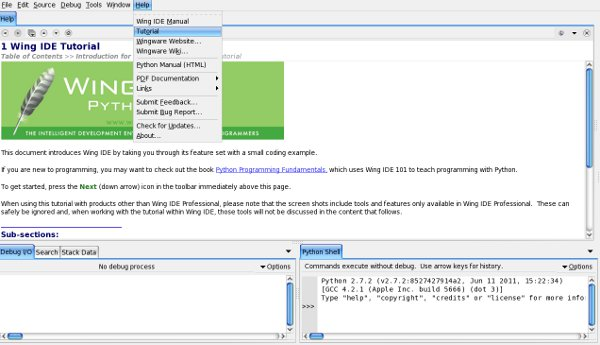
\includegraphics[width=.9\linewidth]{./img/tutorial.jpg}
     \caption{Opening the tutorial in Wing 101.}
     \end{figure}

\end{itemize} % ends low level
\subsection{Further Python Resources}
\label{sec-2-2}


   \textbf{But wait, I want to spend four months becoming a Python guru!}

   Dude, you're awesome.  Here are some resources that will help you:

\begin{itemize}
\item \href{http://knuth.luther.edu/~leekent/IntroToComputing/}{Python Programming Fundamentals}
     Uses WingIDE to teach basic computer science tactics using python
\item \href{http://www.pythonchallenge.com/}{Python Challenge}
     A fun programming riddle that will increase your chops.
\item \href{http://learnpythonthehardway.org/}{Learn Python The Hard Way}
     The Hard Way means by actually writing code.  Maybe it should be
     called The Good Way?
\end{itemize}
\subsection{Diving In}
\label{sec-2-3}

   In Wing, there is a window open called \textbf{Python Shell}   
\begin{itemize}
\item If you know \textbf{R}, think of this just like the R command line
\item If you've never programmed before, think of this as a graphing calculator
\end{itemize}

\begin{minted}[]{python}
print 2+4
\end{minted}

\begin{verbatim}
 6
\end{verbatim}
\subsubsection{Basic Text Handling}
\label{sec-2-3-1}

\begin{itemize}
\item Of course, this graphing calculator can handle text, too!
\end{itemize}

\begin{minted}[]{python}
mystr = "Hello, World!"
print mystr
print len(mystr)
\end{minted}

\begin{verbatim}
 Hello, World!
 13
\end{verbatim}


\begin{center}
\begin{tabular}{lll}
 \textbf{Python Code}              &  \textbf{R Code}                    &  \textbf{English Translation}                                                                                                                                 \\
 \texttt{print 2+4}                &  \texttt{print(2+4)}                &  Print the value of 2+4                                                                                                                                       \\
 \texttt{mystr = '`Hello World'`}  &  \texttt{mystr <- '`Hello World'`}  &  Assign the string ``Hello World'' to the variable mystr                                                                                                      \\
 \texttt{len(mystr)}               &  \texttt{nchar(mystr)}              &  How ``long'' is the variable mystr?  \emph{Note: R can tell you how long it is, but if you want the number of characters, that's what you need to ask for.}  \\
\end{tabular}
\end{center}



\textbf{Note to Stata Users:}\\
Assigning a variable is not the same as adding a ``column'' to your dataset.
\subsubsection{Indexing and Slicing}
\label{sec-2-3-2}

Get the first element of a string.

\begin{itemize}
\item \textbf{Note:} Python counts from 0.  This is a common convention in most
  languages constructed by computer scientists.
\end{itemize}


\begin{minted}[]{python}
mystr = "Dogs in outer space"
print mystr[0]
\end{minted}

\begin{verbatim}
 D
\end{verbatim}

Get the last element of a string

\begin{minted}[]{python}
mystr = "Dogs in outer space"
print mystr[-1]
print mystr[len(mystr)-1]
\end{minted}

\begin{verbatim}
 e
 e
\end{verbatim}


\begin{minted}[]{python}
mystr = "Dogs in outer space"
print mystr[1:3]
print mystr[3:]
print mystr[:-3]
\end{minted}

\begin{verbatim}
 og
 s in outer space
 Dogs in outer sp
\end{verbatim}
\subsubsection{Including Other Packages}
\label{sec-2-3-3}


\begin{itemize}
\item By default, python doesn't include every possible ``package''
\begin{itemize}
\item This is similar to R, but unlike Matlab
\item Use the \texttt{include} statement to load a library
\end{itemize}
\end{itemize}


\begin{minted}[]{python}
import math
print math.sin(math.pi)
\end{minted}

\begin{verbatim}
 1.22464679915e-16
\end{verbatim}

After we import from a package, we have to access sub-elements of that
package using the \texttt{.} operator.  Notice also that while the value
\texttt{1.22464679915e-16} is very nearly \texttt{0}, the \texttt{math} module doesn't know
that $\sin$($\pi$) = 0.  There are smarter modules for doing math in
Python, like \texttt{scipy} and \texttt{numpy}.  Some people love using Python for
Math.  I think it makes more sense to use R.

\begin{itemize}
\item If you want to \texttt{import} something into your namespace
\begin{itemize}
\item \texttt{from math import <myfunction>} \textbf{or}
\item \texttt{from math import *}
\end{itemize}
\end{itemize}


\begin{minted}[]{python}
from math import *
print sin(pi)
\end{minted}

\begin{verbatim}
 1.22464679915e-16
\end{verbatim}
\subsubsection{Objects and methods}
\label{sec-2-3-4}


Python makes extensive use of \textbf{objects}.  An object has
\begin{itemize}
\item Methods: functions that work only on that option
\item Fields: data that only that type of object has
\end{itemize}

For example, let's imagine a \texttt{fruit} object.  A \texttt{fruit} might have a
field called \texttt{hasPeel}, which tells you whether this fruit is
peeled. It could also have a method called \texttt{peel}, which alters the
state of the fruit.


\begin{minted}[]{python}
str = "THE World is A BIG and BEAUTIFUL place.  "
print str.upper()
name = "Alex Storer"
print name.swapcase()
\end{minted}

\begin{verbatim}
 THE WORLD IS A BIG AND BEAUTIFUL PLACE.  
 aLEX sTORER
\end{verbatim}

Here we defined two strings, \texttt{str} and \texttt{name}, and used these to
invoke string methods which affect the case of the string.

\begin{itemize}
\item You can write your own objects and methods
\item Objects can be sub-classes of other objects
\begin{itemize}
\item e.g., a \texttt{psychologist} is a type of \texttt{researcher}, who does
    everything a \texttt{researcher} does but also some other things only
    a \texttt{pyschologist} does.
\end{itemize}
\end{itemize}
\subsubsection{Defining Functions}
\label{sec-2-3-5}


You can write your own functions, pieces of code that can be used to
take specific inputs and give outputs.  You can create a function by
using the \texttt{def} command.


\begin{minted}[]{python}
def square(x):
    return x*x
print square(9)
\end{minted}

\begin{verbatim}
 81
\end{verbatim}

Pay close attention to the \textbf{whitespace} that is used in Python!
Unlike other languages, it is not ignored.  Everything with the same
indentation is in the same level.  Above, the statement \texttt{return x*x}
is part of the \texttt{square} function, but the following line is outside of
the function definition.
\subsubsection{Logical Flow}
\label{sec-2-3-6}

    \begin{figure}[htb]
    \centering
    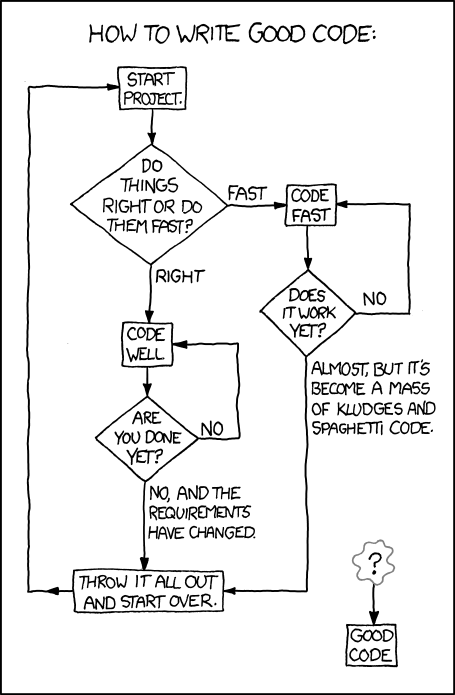
\includegraphics[width=.9\linewidth]{./img/decision-tree.png}
    \caption{The xkcd guide to writing good code}
    \end{figure}

You can think about this logical process as being in pseudocode.

\begin{verbatim}
 IF do things right
    ---> code well
 OTHERWISE
    ---> do things fast
\end{verbatim}

A lot of programming is figuring out how to fit things into this sort
of \texttt{if=/=else} structure.  Let's look at an example in Python.

\begin{itemize}
\item The method \texttt{find} returns the index of the first location of a
  string match
\end{itemize}


\begin{minted}[]{python}
mystr = "This is one cool looking string!"
if mystr.find("string")>len(mystr)/2:
    print "The word 'string' is in the second half"
else:
    print "The word 'string is not in the second half"
\end{minted}

\begin{verbatim}
 The word 'string' is in the second half
\end{verbatim}

What happens if the word ``string'' is not there at all?

\begin{itemize}
\item The method \texttt{find} returns -1 if the string isn't found
\end{itemize}


\begin{minted}[]{python}
mystr = "I don't know about you, but I only use velcro."
print mystr.find("string")
if mystr.find("string")>len(mystr)/2:
    print "The word 'string' is in the second half"
elif mystr.find("string")>=0:
    print "The word 'string is not in the second half"
else:
    print "The word 'string' isn't there!"
\end{minted}

\begin{verbatim}
 -1
 The word 'string' isn't there!
\end{verbatim}

\begin{itemize}
\item \textbf{Important Note:} In Python, most everything evaluates to \texttt{True}.
  Exceptions include \texttt{0} and \texttt{None}.  This means that you can say
  things like \texttt{if (result)} where the result may be a computation, a
  string search, or anything like that.  As long as it evaluates to
  \texttt{True}, it will work!
\end{itemize}
\subsubsection{Review}
\label{sec-2-3-7}

\begin{itemize}
\item \texttt{if}, \texttt{elif} and \texttt{else} can be used to control the flow of a program
\item strings are a type of a object, and have a number of methods that
  come with them, including \texttt{find}, \texttt{upper} and \texttt{swapcase}
\begin{itemize}
\item methods are called using \texttt{mystring.method()}
\item The list of methods for strings can be found in the \href{http://docs.python.org/library/stdtypes.html}{Python documentation}
\end{itemize}
\item \texttt{def} can be used to define a function
\begin{itemize}
\item The \texttt{return} statement determine what the function returns
\end{itemize}
\end{itemize}
\subsection{For Loops}
\label{sec-2-4}

   The for loop is a major component of how python is used.  You can
   iterate over lots of different things, and python is smart enough
   to know how to do it.  
\begin{itemize}
\item \textbf{Note:} the following is what's called pseudocode - something
     that looks like code, but isn't going to run.  It's a helpful way
     to clarify the steps that you need to take to get things to
     work.
\end{itemize}

\begin{minted}[]{python}
for (item in container):
    process item
    print item
print "done processing items!"
\end{minted}


   Notice the use of the <TAB> (or spacing) - that's how python knows whether we're
   inside the loop or not!
\subsubsection{Example}
\label{sec-2-4-1}


\begin{minted}[]{python}
str = "Daddy ran to help Ann.  Up and down went the seesaw."      
for word in str.split():
    print word
\end{minted}


\begin{verbatim}
Daddy
ran
to
help
Ann.
Up
and
down
went
the
seesaw.
\end{verbatim}

    Notice the use of \texttt{str.split()}: this is an example of calling a
    \emph{method} of a \emph{string object}.  It returns a \textbf{list} of words after
    splitting the string on whitespace.
\subsection{Lists}
\label{sec-2-5}


\begin{itemize}
\item A \textbf{list} is a data type that can hold anything.
\item Lists are iterable (you can pass them to a \texttt{for} loop
\item You can \texttt{.append}, \texttt{.extend},and otherwise manipulate lists.  \href{http://docs.python.org/tutorial/datastructures.html}{Python Documentation}
\end{itemize}


\begin{minted}[]{python}
mylist = ['dogs',1,4,"fishes",["hearts","clovers"],list]  
for element in mylist:
    print element    
mylist.reverse()
print mylist
\end{minted}

\begin{verbatim}
 dogs
 1
 4
 fishes
 ['hearts', 'clovers']
 <type 'list'>
 [<type 'list'>, ['hearts', 'clovers'], 'fishes', 4, 1, 'dogs']
\end{verbatim}
\subsection{Exercise}
\label{sec-2-6}

\begin{enumerate}
\item Write a function that takes in a string, and outputs the square of
   its length.
\item Write a function that returns the number of capitalized letters in
   a string. \emph{Hint: try using =lower= and the == operator}
\item Write a function that returns everything in a string up to ``dog'',
   and returns ``not found'' if the string is not present.
\end{enumerate}
\subsubsection{Exercise Solutions}
\label{sec-2-6-1}
\begin{itemize}

\item Exercise 1:\\
\label{sec-2-6-1-1}%
Write a function that takes in a string, and outputs the square of its
length.

Notice that a function can call another function that you wrote.

\begin{minted}[]{python}
def square(x):
    return x*x

def sqlen(x):
    return square(len(x))

print sqlen("Feet")
\end{minted}

\begin{verbatim}
 16
\end{verbatim}


\item Exercise 2\\
\label{sec-2-6-1-2}%
Write a function that returns the number of capitalized letters in a
string.


\begin{minted}[]{python}
def numcaps(x):
    lowerstr = x.lower()
    ncaps = 0
    for i in range(len(x)):
        if lowerstr[i]!=x[i]:
            ncaps += 1
    return ncaps

teststr = "Dogs and Cats are both Animals"
print teststr, "has", str(numcaps(teststr)), "capital letters"
\end{minted}

\begin{verbatim}
 Dogs and Cats are both Animals has 3 capital letters
\end{verbatim}


\item Exercise 3\\
\label{sec-2-6-1-3}%
\begin{minted}[]{python}
def findDog(x):
    mylist = x.split("dog")
    if len(mylist) < 2:
        return "not found"
    else:
        return mylist[0]    
    return mylist
print findDog("i have a dog but not a cat")
print findDog("i have a fish but not a cat")
print findDog("i have a dog but not a dogwood")
\end{minted}

\begin{verbatim}
 i have a 
 not found
 i have a 
\end{verbatim}

\end{itemize} % ends low level
\subsection{\texttt{dict} type}
\label{sec-2-7}

   A \texttt{dict}, short for dictionary, is a helpful data structure in
   Python for building mappings between inputs and outputs.

\href{http://code.google.com/edu/languages/google-python-class/images/dict.png}{http://code.google.com/edu/languages/google-python-class/images/dict.png}
\subsubsection{Examples}
\label{sec-2-7-1}


\begin{minted}[]{python}
mydict = dict()
mydict["dogs"] = 14
mydict["fish"] = "slumberland"
mydict["dogs"]+= 3
print mydict
\end{minted}

\begin{verbatim}
 {'fish': 'slumberland', 'dogs': 17}
\end{verbatim}


\begin{minted}[]{python}
len(mydict["fish"])
\end{minted}


    One of the nice things about python is that even when very
    condensed, it is still readable.  People talk about coding in a
    pythonic way, meaning to write very tight, readable code.


\begin{minted}[]{python}
print dict([(x, x**2) for x in (2, 4, 6)])
\end{minted}

\begin{verbatim}
     {2: 4, 4: 16, 6: 36}
\end{verbatim}

    Let's use a dictionary to store word counts from a sentence.


\begin{minted}[]{python}
str = "Up and down went the seesaw. Up it went.  Down it went.  Up, up, up!"
print str
for i in [",",".","!"]:
    str = str.replace(i," ")
print str
str = str.lower()
print str
print set(str.lower().split())
\end{minted}

\begin{verbatim}
     Up and down went the seesaw. Up it went.  Down it went.  Up, up, up!
     Up and down went the seesaw  Up it went   Down it went   Up  up  up 
     up and down went the seesaw  up it went   down it went   up  up  up 
     set(['and', 'up', 'it', 'down', 'seesaw', 'went', 'the'])
\end{verbatim}

    We see that a \texttt{set} contains an unordered collection of the
    elements of the list returned by \texttt{split()}.  Let's make a dictionary
    with keys that are pulled from this set.


\begin{minted}[]{python}
str = "Up and down went the seesaw. Up it went.  Down it went.  Up, up, up!"
for i in [",",".","!"]:
    str = str.replace(i," ")
words = str.lower().split()
d = dict.fromkeys(set(words),0)
print d
for w in words:
    d[w]+=1
print d
\end{minted}

\begin{verbatim}
     {'and': 0, 'down': 0, 'seesaw': 0, 'went': 0, 'the': 0, 'up': 0, 'it': 0}
     {'and': 1, 'down': 2, 'seesaw': 1, 'went': 3, 'the': 1, 'up': 5, 'it': 2}
\end{verbatim}
\subsubsection{Writing to CSV}
\label{sec-2-7-2}


    A very useful feature of dictionaries is that there is an easy
    method to write them out to a CSV (comma-separated variable) file.


\begin{minted}[]{python}
import csv
f = open('/tmp/blah.csv','w')
nums = [1,2,3]
c = csv.DictWriter(f,nums)
for i in range(0,10):
    c.writerow(dict([(x, x**i) for x in nums]))
f.close()
\end{minted}


    This writes out the following csv file:

\begin{verbatim}
1,1,1
1,2,3
1,4,9
1,8,27
1,16,81
1,32,243
1,64,729
1,128,2187
1,256,6561
1,512,19683
\end{verbatim}
\subsubsection{A Note on File Objects}
\label{sec-2-7-3}


\begin{itemize}
\item Think about file objects like a book
\begin{itemize}
\item If a file is open, you don't want other people to mess with it
\item Files can be opened for reading or writing
\item There are methods to move around an open file
\end{itemize}
\item Close the book when you're done reading it!
\item Python documentation on ``File I/O'' is \href{http://docs.python.org/tutorial/inputoutput.html}{here}
\end{itemize}


\begin{center}
\begin{tabular}{l|l|l}
 English                                  &  Python                             &  Output                           \\
\hline
 Open \texttt{blah.txt} just for reading  &  \texttt{f = open('blah.txt','r')}  &  file object \texttt{f}           \\
 Get the next line in a file              &  \texttt{str = f.readline()}        &  string containing a single line  \\
 Get the entire file                      &  \texttt{str = f.read()}            &  string containing entire file    \\
 Go to the beginning of a file            &  \texttt{f.seek(0)}                 &  \texttt{None}                    \\
 Close \texttt{blah.txt}                  &  \texttt{f.close()}                 &  \texttt{None}                    \\
\end{tabular}
\end{center}



To play with this, download \href{http://www.people.fas.harvard.edu/~astorer/scraping/gaga.txt}{this file} somewhere on your hard drive.
I'm putting it on my hard drive as \texttt{/tmp/gaga.txt}.  On Windows, it
may look more like \texttt{C:\textbackslash{}temp\textbackslash{}gaga.txt} - just make sure you get the
path correct when you tell Python where to look!


\begin{minted}[]{python}
f = open('/tmp/gaga.txt','r')
print f
str = f.read()
print "str has length: ", len(str)
str2 = f.read()
print "str2 has length: ", len(str2)
f.seek(0)
str3 = f.readline()
print "str3 has length: ", len(str3)
f.close()
\end{minted}

\begin{verbatim}
 <open file '/tmp/gaga.txt', mode 'r' at 0x10045e8a0>
 str has length:  1220
 str2 has length:  0
 str3 has length:  77
\end{verbatim}
\subsubsection{Exercise}
\label{sec-2-7-4}
\begin{itemize}

\item Exercise 1\\
\label{sec-2-7-4-1}%
Write a function that counts the number of unique letters in a word.


\item Exercise 2\\
\label{sec-2-7-4-2}%
Write a function that takes in a string, and returns a \texttt{dict} that
tells you how many words of each number of letters there are.
\begin{verbatim}
 "Dogs and cats are all animals"
  dogs and cats are al  animls
  4    3   4    3   2   6
  {2: 1, 3: 2, 4: 2, 6: 1}
\end{verbatim}


\item Exercise 3\\
\label{sec-2-7-4-3}%
Loop over a list of strings, and write a csv that contains a column
for each number and a row for each string.
\begin{verbatim}
  1,2,3,4,5,6,7,8,9,10,11,12,13
  2,3,2,3,4,5,2,3,2,1 , 0, 0, 0
  5,2,1,0,1,2,0,0,0,0 , 0, 0, 0
  etc.
\end{verbatim}

\end{itemize} % ends low level
\subsubsection{Exercise Solutions}
\label{sec-2-7-5}
\begin{itemize}

\item Exercise 1\\
\label{sec-2-7-5-1}%
Write a function that counts the number of unique letters in a word.


\begin{minted}[]{python}
def uniqueletters(w):
    d = dict()
    for char in w:
        d[char] = 1
    return len(d.keys())
print uniqueletters("dog")
print uniqueletters("dogged")
\end{minted}

\begin{verbatim}
 3
 4
\end{verbatim}


\item Exercise 2\\
\label{sec-2-7-5-2}%
Write a function that takes in a string, and returns a \texttt{dict} that
tells you how many words of each number of letters there are.
\begin{verbatim}
 "Dogs and cats are all animals"
  dogs and cats are al  animls
  4    3   4    3   2   6
  {2: 1, 3: 2, 4: 2, 6: 1}
\end{verbatim}


\begin{minted}[]{python}
def uniqueletters(w):
    d = dict()
    for char in w:
        d[char] = 1
    return len(d.keys())

def wordcounter(str):
    d = dict()
    for w in str.split():
        u = uniqueletters(w)
        if u in d.keys():           
            d[u]+=1
        else:
            d[u] = 1
    return d

print wordcounter("Dogs and cats are all animals")
\end{minted}

\begin{verbatim}
 {2: 1, 3: 2, 4: 2, 6: 1}
\end{verbatim}


\item Exercise 3\\
\label{sec-2-7-5-3}%
Loop over a list of strings, and write a csv that contains a column
for each number and a row for each string.
\begin{verbatim}
  1,2,3,4,5,6,7,8,9,10,11,12,13
  2,3,2,3,4,5,2,3,2,1 , 0, 0, 0
  5,2,1,0,1,2,0,0,0,0 , 0, 0, 0
  etc.
\end{verbatim}


\begin{minted}[]{python}
import csv
def uniqueletters(w):
    d = dict()
    for char in w:
        d[char] = 1
    return len(d.keys())

def wordcounter(str):
    d = dict()
    for w in str.split():
        u = uniqueletters(w)
        if u in d.keys():           
            d[u]+=1
        else:
            d[u] = 1
    return d

def listwriter(l):
    emptydict = dict([(x, 0) for x in range(1,26)])
    f = open('/tmp/blah.csv','w')
    c = csv.DictWriter(f,sorted(emptydict.keys())) 
    c.writeheader()    
    for str in l:
        c.writerow(dict(emptydict.items()+wordcounter(str).items()))
    f.close()

listwriter(["Five score years ago, a great American, in whose symbolic shadow we stand today, signed the Emancipation Proclamation.",
            "We observe today not a victory of party, but a celebration of freedom -- symbolizing an end, as well as a beginning -- signifying renewal, as well as change.", 
            "So, first of all, let me assert my firm belief that the only thing we have to fear is fear itself -- nameless, unreasoning, unjustified terror which paralyzes needed efforts to convert retreat into advance."])
\end{minted}


Here is the resulting CSV file:
CANNOT INCLUDE FILE /tmp/blah.csv

\end{itemize} % ends low level
\section{Regular Expressions}
\label{sec-3}


Regular expressions are a framework for doing complicated
manipulation.  
\subsection{A first example}
\label{sec-3-1}


For example, consider the following text:
\begin{verbatim}
 Joseph Schmoe (15), Phone:(934) 292-2390, SSN:295-48-2019
\end{verbatim}
A first guess for a rule to get the area code would be to find a
grouping of three numbers.
Let's look at the source code for this in python.


\begin{minted}[]{python}
import re  
str = "Joseph Schmoe (15), Phone:(934) 292-2390, SSN:295-48-2311"  
print re.findall("\d\d\d",str)
\end{minted}

\begin{verbatim}
 ['934', '292', '239', '295', '231']
\end{verbatim}
\subsubsection{What the code does}
\label{sec-3-1-1}

\begin{itemize}
\item \texttt{import re}
\begin{itemize}
\item tells python to use the regular expression library.  (Like \texttt{library(zelig)})
\end{itemize}
\item \texttt{str = ...}
\begin{itemize}
\item defines a string
\item Python will figure out that the type is a string based on the fact that it's in quotes
\item There is a difference between
\begin{verbatim}
      foo = '333'
\end{verbatim}
     and
\begin{verbatim}
      foo = 333
\end{verbatim}
\end{itemize}
\item \texttt{re.findall("\textbackslash{}d\textbackslash{}d\textbackslash{}d",str)}
\begin{itemize}
\item From the \texttt{re} library, call the \texttt{findall} function
\begin{itemize}
\item When in doubt, \href{https://www.google.com/search?sourceid=chrome&ie=UTF-8&q=re.findall}{Google it}.
\begin{itemize}
\item \emph{By the way, googling things effectively is the most important          modern research skill there is.}
\end{itemize}
\end{itemize}
\item Finds all of the matched of the regular expression \texttt{\textbackslash{}d\textbackslash{}d\textbackslash{}d} in \texttt{str}
\begin{itemize}
\item Returns it as a list
\end{itemize}
\end{itemize}
\end{itemize}


\begin{minted}[]{python}
import re
str = "Joseph Schmoe (15), Phone:(934) 292-2390, SSN:295-48-2311"  
print re.findall("\((\d\d\d)\)",str)
\end{minted}

\begin{verbatim}
 ['934']
\end{verbatim}

    
\subsubsection{Different expressions}
\label{sec-3-1-2}

\begin{verbatim}
 "Joseph Schmoe (15), Phone:(934) 292-2390, SSN:295-48-2311"  
\end{verbatim}

\begin{center}
\begin{tabular}{l|l|l}
 English                                                   &  Regex                                                                                             &  \texttt{findall} Output                              \\
\hline
 Any three numbers                                         &  \texttt{\textbackslash{}d\textbackslash{}d\textbackslash{}d}                                      &  \texttt{['934', '292', '239', '295', '231']}         \\
 Any three numbers that start with (                       &  =\(\d\d\d=                                                                                        &  =['(934']=                                           \\
 One or more adjacent numbers                              &  =\d+=                                                                                             &  =['15', '934', '292', '2390', '295', '48', '2311']=  \\
 One or more numbers in parenthesis                        &  \texttt{\textbackslash{}(\textbackslash{}d+\textbackslash{})}                                     &  \texttt{['(15)', '(934)']}                           \\
 Three numbers in parenthesis                              &  \texttt{\textbackslash{}(\textbackslash{}d\textbackslash{}d\textbackslash{}d\textbackslash{})}    &  \texttt{['(934)']}                                   \\
 Three numbers in parenthesis, but group only the numbers  &  \texttt{\textbackslash{}((\textbackslash{}d\textbackslash{}d\textbackslash{}d)\textbackslash{})}  &  \texttt{['934']}                                     \\
\end{tabular}
\end{center}


    
\subsection{Further examples}
\label{sec-3-2}


\begin{minted}[]{python}
import re
str = "Joseph Schmoe, Bowling High Score:(225), Phone:(934) 292-2390"  
print re.findall("\w+:\((\d+)\)",str)
\end{minted}

\begin{verbatim}
    ['225', '934']
\end{verbatim}

\begin{itemize}
\item The \texttt{\textbackslash{}w} is code for any alphanumeric character and the underscore.
\item The \texttt{:} is code for only the character \texttt{:}.
\end{itemize}


\begin{minted}[]{python}
import re
str = "I called his phone after he phoned me, but he has two phones!"  
print re.findall("phone\w*",str)
\end{minted}

\begin{verbatim}
    ['phone', 'phoned', 'phones']
\end{verbatim}

\begin{itemize}
\item We match all instances of ``phone'' with any number of characters
     after it
\begin{itemize}
\item Note the difference between \texttt{\textbackslash{}w+} (1 or more) and \texttt{\textbackslash{}w*} (0 or more)
\end{itemize}
\end{itemize}


\begin{minted}[]{python}
import re
str = "I called his phone after he phoned me, but he has two phones!"  
print re.findall("phone\w+",str)
\end{minted}

\begin{verbatim}
    ['phoned', 'phones']
\end{verbatim}

   
\subsection{Other helpful regex tools}
\label{sec-3-3}

Regular expressions are extremely powerful, and are used extensively
for text processing.  Here are some good places to look for regex help:
\begin{itemize}
\item \href{http://docs.python.org/library/re.html}{Python re library} has documentation of how to use regex in python with
  examples
\begin{itemize}
\item \emph{I can never remember regex syntax, so I go here all the time.}
\end{itemize}
\item \href{http://gskinner.com/RegExr/}{Regexr} is an interactive regex checker
\item Textbooks on regex will tell you not just how to use them, but how
  they are implemented.  Help answer the question ``what is the best
  regex for this situation?''
\end{itemize}
\subsection{Exercise}
\label{sec-3-4}


\href{file:///Users/astorer/Work/presentations/scraping/example.txt}{This file} contains 100 blogs about dogs in a structured text
format that may be familiar to you.  Use regular expressions to parse
this file and write a csv file containing the article number and
the number of words.  (I'm going to start by downloading it to my hard
drive, but if you're macho you can figure out how to use the \texttt{urllib}
module to parse it without downloading.  If this is a breeze, try to
parse out the title, too.  Make sure you double check that you got it right!)
\subsubsection{Solution}
\label{sec-3-4-1}



\begin{minted}[]{python}
import csv, re
f = open('/tmp/example.txt')
fp = open('/tmp/result.csv','wb')

c = csv.DictWriter(fp,["Article Number","Words"]) 
articlenum = 0
for line in f:
    d = dict()
    r = re.match("LENGTH:\s*(\d+)",line)
    if r:
        articlenum+=1
        d["Article Number"] = articlenum
        d["Words"] = r.groups()[0]
        c.writerow(d)        
f.close()
fp.close()
\end{minted}


The \texttt{result.csv} file is:
CANNOT INCLUDE FILE /tmp/result.csv
\section{Web Sites}
\label{sec-4}
\subsection{Example: Egypt Independent / المصري اليوم}
\label{sec-4-1}

\begin{itemize}
\item Example article: \href{http://www.egyptindependent.com/node/725861}{http://www.egyptindependent.com/node/725861}
\begin{itemize}
\item Tells us nothing about the date or content
\item A node number is automatically created by a content-management
    system
\end{itemize}
\end{itemize}
\subsubsection{Metadata}
\label{sec-4-1-1}

Sometimes, metadata is included which tells us important things
about our article

\begin{minted}[]{html}
<meta http-equiv="Content-Type" content="text/html; charset=utf-8" />
<meta name="msvalidate.01" content="F1F61CF0E5EC4EC2940FCA062AB13A53" />
<meta name="google-site-verification" content="Q8FKHdNoQ2EH7SH1MzwH_JNcgVgMYeCgFnzNlXlR4N0" />
<title>European Union will keep Mubarak assets on ice, Illicit Gains Authority head says | Egypt Independent</title>
<!-- tC490Uh18j-7O_rp7nG0_e6U9QY -->
<meta http-equiv="Content-Type" content="text/html; charset=utf-8" />
<link rel="canonical" href="http://www.egyptindependent.com/node/725861" />
<meta name="keywords" content="Assem al-Gohary, corruption, EU, freezing  Mubarak’s assets, Hosni Mubarak, Illicit Gains Authority (IGA), News, Top stories" />
<meta name="description" content="The European Union will continue to freeze the assets of former President Hosni Mubarak, his family and other former officials although Egypt has thus far been unsuccessful in recovering funds siphoned abroad by the regime." />
<meta name="abstract" content="Al-Masry Al-Youm - Egypt&#039;s leading independent media group المصرى اليوم للصحافة والنشر هى مؤسسة إعلامية مصرية مستقلة تأسست عام  ,2003." />
\end{minted}
\begin{itemize}
\item Keywords, abstract, description and title are all clear
\item Lots of other gunk that isn't relevant to us!
\item Pulling information out of this document requires that we know how
    they organize title their metadata!
\begin{itemize}
\item What if \emph{keywords} were called \emph{terms}?
\end{itemize}
\end{itemize}
\subsubsection{Body}
\label{sec-4-1-2}

The actual body of the article can be found by right-clicking on the
  text we're interested in from Chrome or Firefox and selecting
  ``Insepct Element''

\begin{minted}[]{html}
<div class="panel-region-separator"></div><div class="panel-pane pane-node-body" >    
  <div class="pane-content">
    <p>The European Union will continue to freeze the assets of former President Hosni Mubarak, his family and other former officials although Egypt has thus far been unsuccessful in recovering funds siphoned abroad by the regime.</p>
<p>The Illicit Gains Authority (IGA), the judicial committee responsible for recovering the money, on Wednesday received an official notification from the European Union, confirming its freeze on the assets would be renewed another year as of 19 March, state-run MENA news service reported on Wednesday.&nbsp;</p>
<p>&ldquo;This was in response to a request by Egypt,&rdquo; the state news agency quoted IGA head Assem al-Gohary as saying.&nbsp;</p>
<p>Egypt formally asked European Union countries earlier this month to continue freezing funds belonging to Mubarak, his two sons and other members of his administration.</p>
<p>Shortly after Mubarak was forced to step down in February 2011, the public prosecutor ordered that the foreign assets of the deposed president and his family be frozen.</p>
<p>Mubarak&#39;s actual worth is still unknown after more than a year of investigations into his foreign and domestic assets. Last year claims that Mubarak, in his nearly 30-year reign as head of state, may have amassed a fortune of up to US$70 billion &mdash; greater than that of Microsoft&#39;s Bill Gates &mdash; helped drive the protests that eventually brought him down.</p>
<p>Last year Swiss authorities also froze Mubarak&rsquo;s assets, acting more speedily than when the EU froze the assets of another deposed North African ruler, former Tunisian President Zine al-Abidine Ben Ali.</p>
<p>On Wednesday, the IGA met with the Swiss ambassador in Cairo to discuss the difficulties it faces in recovering those funds, in light of the obligations of the United Nations Convention Against Corruption on the member states, reported MENA.</p>
<p>Gohary once estimated the frozen assets at 410 million Swiss francs (LE2.7 billion), which Egypt is trying to repatriate in cooperation with the Foreign Ministry.</p>
  </div>
\end{minted}
All of the body is included in the \texttt{panel-pane pane-node-body} section
of this site, within the sub-section \texttt{pane-content}.  Our ``algorithm''
for getting this information out will require finding the exact
section of the site that we require pulling this data out from.  If
you don't do this, any terms that are on the sidebar will end up being
in your analysis!
\subsubsection{Scraping Articles}
\label{sec-4-1-3}


Every News Feature is on a page in the following scheme:


\begin{minted}[]{html}
http://www.egyptindependent.com/subchannel/News%20features?page=5
\end{minted}

And this paper goes back 77 pages, to April, 2009.

Investigating the source for a single search page can tell us what we
have to do to get at the relevant information:


\begin{minted}[]{html}
<div class="views-row views-row-4 views-row-even">
  <div class="views-field-field-published-date-value">
    <span class="field-content"><span class="date-display-single">09 Feb 2012</span></span>
  </div>
  <div class="views-field-title">
    <span class="field-content"><a href="http://www.egyptindependent.com/node/647936">Parliament Review: A week of comedy and disappointment</a></span>
  </div> 
  <div class="views-field-body">
    <span class="field-content">This week&rsquo;s parliamentary sessions had the public joking about airing future sessions on comedy channels instead of news, and those who abstained from the polls telling those who participated, in hope of having a legitimate authority...</span>
  </div>
\end{minted}

Our algorithm to scrape articles from this page will be as follows:
\begin{enumerate}
\item Initialize FOO=1
\item Go to
   \texttt{http://www.egyptindependent.com/subchannel/News\%20features?page=FOO}
\item Repeat until complete:
\begin{enumerate}
\item Find the next occurence of \texttt{views-row...}
\item Find the sub-field called
      \texttt{views-field-field-published-date-value} and retrieve its value
      (the date)
\item Find the sub-field called \texttt{views-field-title} and retrieve its
      value (the title)
\item Follow the link from above
\item Within the link, find the meta-data \texttt{keywords} and retrieve
      their values (the keywords)
\item Within the link, find the \texttt{panel-pane pane-node-body} section,
      and retrieve the test (the article itself)
\end{enumerate}
\end{enumerate}
\section{Implementing the scraper in python}
\label{sec-5}

Now that we know how we want to scrape and have some grasp on the
tools that are necessary, let's try and pull the articles and their
metadata off of this website.
\subsection{Downloading files in python}
\label{sec-5-1}

==
\begin{minted}[]{python}
import urllib
baseurl = "http://www.egyptindependent.com/subchannel/News%20features?page="
destpath = "/tmp/"
npages = 1
for i in range(1,npages):
    urllib.urlretrieve (baseurl+str(i),destpath+"page"+str(i)+".html")
\end{minted}

   If we take a look at what exists after running this script, we can
   see that it worked.


\begin{verbatim}
bash-3.2$ ls /tmp/page*
/tmp/page1.html      /tmp/page3.html /tmp/page5.html /tmp/page7.html /tmp/page9.html
/tmp/page2.html      /tmp/page4.html /tmp/page6.html /tmp/page8.html
\end{verbatim}
\subsection{Using ElementTree}
\label{sec-5-2}


   Here is a very basic html tree which we can work with.


\begin{minted}[]{python}
fileloc = '/Users/astorer/Work/presentations/scraping/test.html'
f = open(fileloc,'r')
print f.read()
\end{minted}


\begin{verbatim}
<html>
    <head>
        <title>Example page</title>
    </head>
    <body>
        <p>Moved to <a href="http://example.org/">example.org</a>
        or <a href="http://example.com/">example.com</a>.</p>
    </body>
</html>
\end{verbatim}


\begin{itemize}
\item The ElementTree is a hierarchical structure of Elements.
\item \texttt{list()} returns a list of the children of a single Element
\item An \href{http://docs.python.org/library/xml.etree.elementtree.html#xml.etree.ElementTree.Element}{Element} contains
\begin{itemize}
\item A \texttt{tag} (what kind of element is it)
\item \texttt{text} of what lives in the element
\end{itemize}
\end{itemize}


\begin{minted}[]{python}
from xml.etree.ElementTree import ElementTree
fileloc = '/Users/astorer/Work/presentations/scraping/test.html'
tree = ElementTree()
tree.parse(fileloc)   
elem = tree.find('body')
print elem
print list(elem)
elem = tree.find('body/p')
print elem
print list(elem)
print elem.tag
print elem.text
\end{minted}

\begin{verbatim}
 <Element 'body' at 0x1004c5310>
 [<Element 'p' at 0x1004c5350>]
 <Element 'p' at 0x1004c5350>
 [<Element 'a' at 0x1004c5390>, <Element 'a' at 0x1004c53d0>]
 p
 Moved to 
\end{verbatim}
\subsection{Using \texttt{lxml}}
\label{sec-5-3}


   Now let's see how we can parse out the list of article URLs from
   an xml page.  Our basic approach isn't going to work here, and we
   need to install an external package.
\subsubsection{Installing a Package}
\label{sec-5-3-1}

    
    External packages can be easily installed in python using the
    \texttt{easy\_install} command.  The only challenge is in making sure that
    if you have multiple version of python installed, you are
    installing the libraries to the correct location.  I'm on a mac,
    but the Python version on a mac is 2.6, and I prefer using 2.7.
    Make sure you install the setuptools for 2.7 following
    \href{http://pypi.python.org/pypi/setuptools}{these instructions}.  Then, run

\begin{verbatim}
     sudo easy_install-2.7 lxml
\end{verbatim}
    
    If you have no idea what I'm talking about, it will probably be
    fine if you simply use the following:

\begin{verbatim}
     sudo easy_install lxml
\end{verbatim}

    To verify that this installed for you, open up python, and type

\begin{verbatim}
     import lxml
\end{verbatim}

    If you get an error, sheck your setup and try reinstalling.
    
\subsubsection{Using \texttt{lxml}}
\label{sec-5-3-2}


    \texttt{lxml} will generate an ElementTree for us after parsing the xml.
    Let's review some of the functions that will be useful for us in
    this example.


\begin{center}
\begin{tabular}{l|l}
 English                                         &  Python                                        \\
\hline
 Construct a parser                              &  \texttt{lxml.etree.HTMLParser()}              \\
 Parse an HTML file                              &  \texttt{lxml.etree.parse(file,parser)}        \\
 Get all instances of \verb~<span class="...">~  &  \verb~MyTree.xpath('.//span[@class="..."]')~  \\
 Make a list of tuples that we can iterate over  &  \texttt{zip(iterable1,iterable2,...)}         \\
 Encode a string \verb~foo~ as unicode (UTF-8)   &  \verb~foo.encode("UTF-8")~                    \\
\end{tabular}
\end{center}



    The \texttt{xpath} syntax is described in more detail \href{http://effbot.org/zone/element-xpath.htm}{here}.  Briefly, we
    are finding every occurence of spans with the class
    \texttt{date-display-single}, no matter where they live in the tree.
    Then we can iterate over them to get the actual dates.  Similarly,
    we can iterate over all links that are within the \verb~<span     class="field content">~ that are within the \verb~<div     class="views-field-title">~ and zip it with the dates to iterate
    over both simultaneously.  Notice that whenever foreign characters
    are used, Python will be unable to display them unless we encode
    the string first as unicode.  The following code makes this explicit.


\begin{minted}[]{python}
from lxml import etree
fname = '/tmp/page1.html'
fp = open(fname, 'rb')
parser = etree.HTMLParser()
tree   = etree.parse(fp, parser)
dateelems = tree.xpath('.//span[@class="date-display-single"]')
linkelems = tree.xpath('.//div[@class="views-field-title"]/span[@class="field-content"]/a')     
for (d,l) in zip(dateelems,linkelems):
    print d.text
    print l.get('href')         
    print l.text.encode("utf-8")
\end{minted}


\begin{verbatim}
27 Mar 2012
http://www.egyptindependent.com/node/736356
Secular forces withdraw from constituent assembly, but next step unclear
26 Mar 2012
http://www.egyptindependent.com/node/735431
Old tensions between Brotherhood and SCAF resurface in game of chicken
23 Mar 2012
http://www.egyptindependent.com/node/728621
Parliament Review: Constitutional mayhem and critical legislation
22 Mar 2012
http://www.egyptindependent.com/node/727691
Path set by constitutional referendum seems unlikely
21 Mar 2012
http://www.egyptindependent.com/node/726096
Meet your presidential candidates: The outsiders
21 Mar 2012
http://www.egyptindependent.com/node/723986
Meet your presidential candidate: Abul Ezz al-Hariry, the rabble rouser
20 Mar 2012
http://www.egyptindependent.com/node/724126
With tears and crowds, Copts say goodbye to Shenouda
19 Mar 2012
http://www.egyptindependent.com/node/722396
Unofficial Abouel Fotouh supporters lay foundation for official campaign
19 Mar 2012
http://www.egyptindependent.com/node/721161
Copts fear implications after Shenouda, disagree on papal political role
19 Mar 2012
http://www.egyptindependent.com/node/720471
Women's movement: A stop at Egypt's socialist era
\end{verbatim}
\subsubsection{Downloading articles from each page}
\label{sec-5-3-3}

    \textbf{Goal:} A file with the dates, titles and location of each
     article.  Save each article in html form to the hard drive.

\begin{minted}[]{python}
from lxml import etree
import csv     
import urllib
import re
f = open('/tmp/files.csv','w')
entries = ["Day","Month","Year","Title","Remote","Local"]
c = csv.DictWriter(f,entries)


destpath = '/tmp/'
fname = '/tmp/page1.html'
fp = open(fname, 'rb')
parser = etree.HTMLParser()
tree   = etree.parse(fp, parser)
dateelems = tree.xpath('.//span[@class="date-display-single"]')
linkelems = tree.xpath('.//div[@class="views-field-title"]/span[@class="field-content"]/a')
for (d,l) in zip(dateelems,linkelems):
    entry = dict()
    myDate = d.text.split()
    urlname = l.get('href')
    nodenum = re.search("\d+",urlname).group()
    dest = destpath+nodenum+".html"
    urllib.urlretrieve (urlname,dest)
    entry["Day"] = myDate[0]
    entry["Month"] = myDate[1]
    entry["Year"] = myDate[2]
    entry["Local"] = dest
    entry["Remote"] = urlname
    entry["Title"] = l.text.encode("utf-8")
    c.writerow(entry)
    print entry

f.close()
fp.close()
\end{minted}


\begin{verbatim}
{'Remote': 'http://www.egyptindependent.com/node/736356', 'Title': 'Secular forces withdraw from constituent assembly, but next step unclear', 'Month': 'Mar', 'Year': '2012', 'Local': '/tmp/736356.html', 'Day': '27'}
{'Remote': 'http://www.egyptindependent.com/node/735431', 'Title': 'Old tensions between Brotherhood and SCAF resurface in game of chicken', 'Month': 'Mar', 'Year': '2012', 'Local': '/tmp/735431.html', 'Day': '26'}
{'Remote': 'http://www.egyptindependent.com/node/728621', 'Title': 'Parliament Review: Constitutional mayhem and critical legislation', 'Month': 'Mar', 'Year': '2012', 'Local': '/tmp/728621.html', 'Day': '23'}
{'Remote': 'http://www.egyptindependent.com/node/727691', 'Title': 'Path set by constitutional referendum seems unlikely', 'Month': 'Mar', 'Year': '2012', 'Local': '/tmp/727691.html', 'Day': '22'}
{'Remote': 'http://www.egyptindependent.com/node/726096', 'Title': 'Meet your presidential candidates: The outsiders', 'Month': 'Mar', 'Year': '2012', 'Local': '/tmp/726096.html', 'Day': '21'}
{'Remote': 'http://www.egyptindependent.com/node/723986', 'Title': 'Meet your presidential candidate: Abul Ezz al-Hariry, the rabble rouser', 'Month': 'Mar', 'Year': '2012', 'Local': '/tmp/723986.html', 'Day': '21'}
{'Remote': 'http://www.egyptindependent.com/node/724126', 'Title': 'With tears and crowds, Copts say goodbye to Shenouda', 'Month': 'Mar', 'Year': '2012', 'Local': '/tmp/724126.html', 'Day': '20'}
{'Remote': 'http://www.egyptindependent.com/node/722396', 'Title': 'Unofficial Abouel Fotouh supporters lay foundation for official campaign', 'Month': 'Mar', 'Year': '2012', 'Local': '/tmp/722396.html', 'Day': '19'}
{'Remote': 'http://www.egyptindependent.com/node/721161', 'Title': 'Copts fear implications after Shenouda, disagree on papal political role', 'Month': 'Mar', 'Year': '2012', 'Local': '/tmp/721161.html', 'Day': '19'}
{'Remote': 'http://www.egyptindependent.com/node/720471', 'Title': "Women's movement: A stop at Egypt's socialist era", 'Month': 'Mar', 'Year': '2012', 'Local': '/tmp/720471.html', 'Day': '19'}
\end{verbatim}


\begin{verbatim}
{'Remote': 'http://www.egyptindependent.com/node/720426', 'Title': "Shenouda leaves Copts divided on his legacy and church's future", 'Month': 'Mar', 'Year': '2012', 'Local': '/tmp/720426.html', 'Day': '18'}
{'Remote': 'http://www.egyptindependent.com/node/718906', 'Title': 'The embattled new National Council for Women', 'Month': 'Mar', 'Year': '2012', 'Local': '/tmp/718906.html', 'Day': '18'}
{'Remote': 'http://www.egyptindependent.com/node/718491', 'Title': 'Who is the pope\xe2\x80\x99s successor?', 'Month': 'Mar', 'Year': '2012', 'Local': '/tmp/718491.html', 'Day': '18'}
{'Remote': 'http://www.egyptindependent.com/node/715431', 'Title': 'Parliament Review: Chasing a turbulent policeman and a vote of no-confidence', 'Month': 'Mar', 'Year': '2012', 'Local': '/tmp/715431.html', 'Day': '16'}
{'Remote': 'http://www.egyptindependent.com/node/714506', 'Title': "SCAF's investment law offers impunity in corruption cases", 'Month': 'Mar', 'Year': '2012', 'Local': '/tmp/714506.html', 'Day': '15'}
{'Remote': 'http://www.egyptindependent.com/node/713231', 'Title': 'What\xe2\x80\x99s left of Tahrir today', 'Month': 'Mar', 'Year': '2012', 'Local': '/tmp/713231.html', 'Day': '14'}
{'Remote': 'http://www.egyptindependent.com/node/711221', 'Title': "Students object to minister's intervention in university bylaws", 'Month': 'Mar', 'Year': '2012', 'Local': '/tmp/711221.html', 'Day': '13'}
{'Remote': 'http://www.egyptindependent.com/node/707721', 'Title': 'Meet your presidential candidate: Mansour Hassan, the resuscitated', 'Month': 'Mar', 'Year': '2012', 'Local': '/tmp/707721.html', 'Day': '12'}
{'Remote': 'http://www.egyptindependent.com/node/707961', 'Title': 'GUC strike moves protest to new territory, private universities', 'Month': 'Mar', 'Year': '2012', 'Local': '/tmp/707961.html', 'Day': '12'}
{'Remote': 'http://www.egyptindependent.com/node/707556', 'Title': '\xe2\x80\x98Virginity test\xe2\x80\x99 doctor acquittal reveals military judiciary shortcomings', 'Month': 'Mar', 'Year': '2012', 'Local': '/tmp/707556.html', 'Day': '11'}
\end{verbatim}

The resulting file is a CSV file.:
CANNOT INCLUDE FILE /tmp/files.csv
\subsubsection{Exercise}
\label{sec-5-3-4}


Modify the above code so that instead of iterating over only the first page, it iterates over all pages.

\begin{itemize}
\item Consider using the \texttt{glob} library to look for all of the html files in a directory.
\item Can you do this so you don't save the pages, but parse them directly?
\begin{itemize}
\item Use google and the python documentation to help figure it out!
\end{itemize}
Now that we've seen \texttt{lxml} in action, let's figure out how to use
   it to pull out just the text of the article.  Recall that
   all of the original text is in the following tags:
   
\begin{verbatim}
    <div class="panel-pane pane-node-body" >    
    <div class="pane-content">
\end{verbatim}
\end{itemize}
     
\subsection{Stripping text}
\label{sec-5-4}

\end{document}
